\section{Problema 3}

\subsection{Definizione dei sottoproblemi}

Nella risoluzione del problema, abbiamo focalizzato il nostro ragionamento sulla proprietà fondamentale che deve avere un albero per
essere accettabile, ovvero:
\begin{itemize}
	\item Il costo complessivo dell'albero deve essere minimo.
	\item Ogni nodo interno deve avere esattamente due figli.
	\item L'albero ha  esattamente $n$ foglie.
\end{itemize}

\begin{center}
	\textbf{$OPT[i, j]$ rappresenta l'albero di costo minimo contenente le foglie $\{C[j], C[j + 1], ..., C[j + i - 1]\}$ date in input, 
		$\forall i\ \in\ \{1, ..., n\} \land \forall j\ \in\ \{1, ..., n - i + 1\}$ dove $i$ indica la $i-esima$ riga e $j$ indica la $j-esima$ colonna della matrice $OPT$.}
\end{center}

\subsection{Struttura dati}

Abbiamo definito una matrice $OPT$ di dimensioni $n \times n$, dove ogni cella contiene 4 valori:

\begin{itemize}
	\item $OPT[i, j].val$: il costo minimo per costruire un albero con le foglie che vanno da $j$ a $j + i - 1$ (dove $i$ rappresenta le righe e $j$ le colonne).
	\item $OPT[i, j].max$: il valore massimo tra le foglie all'interno dell'intervallo $[j: j + i - 1]$.
	\item $OPT[i, j].sin$: le coppie di indici $i,\ j$ che all'interno di $OPT$ ci indicano quale cella guardare per ricostruire la struttura del sottoalbero sinistro.
	\item $OPT[i, j].des$: le coppie di indici $i,\ j$ che all'interno di $OPT$ ci indicano quale cella guardare per ricostruire la struttura del sottoalbero destro.
\end{itemize}

Tuttavia, è importante notare che utilizziamo solo la metà delle celle di $OPT$. In particolare,
ci limitiamo alla matrice triangolare superiore sinistra, poiché oltre questa 
zona andremmo oltre il numero di foglie salvate nell'array $C$, che contiene i valori delle foglie dati in input.

\subsection{Combinazione dei sottoproblemi}

Nel processo di combinazione dei sottoproblemi, abbiamo tenuto presente che un albero ottimale deve essere strutturato in modo binario, cioè deve avere due 
sottoalberi per ogni nodo interno. Questa considerazione ci ha portato a distinguere le foglie in due gruppi: le "foglie destre", che appartengono al sottoalbero 
destro, e le "foglie sinistre", che appartengono al sottoalbero sinistro.

\subsubsection*{Casi base}

Durante l'analisi dei casi base, abbiamo individuato due situazioni:

\begin{itemize}
	\item {
		Il primo caso base riguarda la prima riga della matrice, che rappresenta una foglia singola. In questo caso, assegniamo il valore della foglia a $OPT[1, j].max$, 
		mentre poniamo il valore di $OPT[1, j].val = 0$ (poiché per la nostra definizione le foglie non hanno valore). $OPT[1, j].sin$ e $OPT[1, j].des$ non vengono inizializzate in quanto 
		non ci sono sottoalberi.
	}
	\item {
		Il secondo caso base si riferisce alla seconda riga della matrice, che rappresenta un albero con solo due foglie. Questo albero può essere combinato in un 
		unico modo, poiché le foglie devono essere ordinate secondo una visita simmetrica rispetto all'input. In questo caso, il valore di $OPT[2, j].val$ è il prodotto tra 
		gli $OPT[1, j].max$ e $OPT[1, j + 1].max$ i quali indicano le foglie, mentre $OPT[2, j].max$ rappresenta il massimo tra i due valori delle foglie. Inoltre, assegniamo gli indici delle foglie a $OPT[2, j].sin$ e $OPT[2, j].des$ 
		per poter trovare facilmente le loro posizioni nella matrice.
	}
\end{itemize}

\subsubsection*{Caso generico}

Avendo effettuato questa suddivisione tra sottoalbero destro e sottoalbero sinistro, ci siamo resi conto che la chiave per trovare il valore dell'albero 
ottimale consiste nel provare tutte le possibili suddivisioni fra foglie destre e sinistre e trovare quella con il costo complessivo minimo. Questo si riduce a 
cercare un indice $k$ nell'intervallo $[1 : i - 1]$ tale che il nodo risultante dalla combinazione del sottoalbero sinistro contenente le foglie da $j$ a $j + k$ e del 
sottoalbero destro contenente le foglie da $j + k +1$ a $j + i - 1$ sia il più piccolo possibile in termini di costo.

\newpage
\subsubsection*{Goal}

Il valore dell'albero minimo che stiamo cercando si trova all'interno della cella $OPT[n,1].val$. 
Questa cella contiene il valore dell'albero minimo che include tutte le foglie che vanno da 
$C[1]$ a $C[n]$ (essendo $i = 1$ e $j = n$). 
Poiché questo albero contiene tutte le foglie, è l'albero di costo minimo che stiamo cercando.

\subsection{Formula di Bellman}

\subsubsection*{Caso base, $i = 1$}

\begin{align*}
	OPT[i, j]	
	\begin{cases}
		.val = 0\\                                                                                          
		.max = C[j]\\
		.sin = NULL\\
		.des = NULL\\
	\end{cases}                                                                                            
\end{align*}


\subsubsection*{Caso base, $i = 2$}

\begin{align*}
	OPT[i, j]	
	\begin{cases}
		.val = OPT[i - 1, j].max \times OPT[i - 1, j + 1].max\\                                                                                          
		.max = \max\{OPT[i - 1, j].max, OPT[i - 1, j + 1].max\}\\
		.sin = (i - 1, j)\\
		.des = (i - 1, j + 1)\\
	\end{cases}                                                                                            
\end{align*}

\subsubsection*{Caso generico}

$$
OPT[i, j].val = \min_{1 \leq k \leq i - 1}\{(OPT[i - k, j].max \times OPT[k, i - k + j].max) + 											OPT[i - k, j].val + OPT[k, i - k + j].val\}
$$

Dopo aver trovato il $k$ che minimizza la formula sopra, calcoliamo i restanti 3 campi di $OPT[i, j]$

\begin{align*}
	OPT[i, j]	
	\begin{cases}                                                                                          
		.max = \max\{(OPT[i - k, j].max, OPT[k, i - k + j].max)\}\\
		.sin = (i - k, j)\\
		.des = (k, i - k + j)\\
	\end{cases}                                                                                            
\end{align*}



\subsubsection*{Esempio}

Supponiamo di avere in input il seguente vettore $C = [4, 2, 7]$ con 3 foglie.

Ogni cella della matrice contiene 4 valori, dunque possiamo codificare questi 4 valori come 
il seguente array: $[.val, .max, .sin, .des]$.

\[
	\begin{bmatrix}
		[0, 4, -, -]           & [0, 2, -, -]            & [0, 7, -, -] \\
		[8, 4, (1, 1), (1, 2)] & [7, 14, (1, 2), (1, 3)] & [-, -, -, -] \\
		[?, ?, ?, ?]           & [-, -, -, -]            & [-, -, -, -] \\
	\end{bmatrix}
\]

Per riempire la cella $OPT[3, 1]$, che contiene il valore dell'albero minimo, 
dobbiamo determinare la combinazione ottimale delle foglie che produce l'albero di costo minimo. 
Quindi, dobbiamo trovare l'indice $k$ compreso tra $1$ e $i - 1$. Considerando la cella $(3, 1)$, 
dove $i = 3$, i possibili valori per $k$ sono $1$ e $2$.


\begin{center}
	\begin{enumerate*}[label={}]
	\item {
		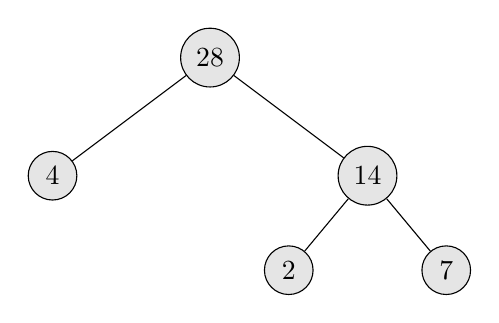
\begin{tikzpicture}[
				level/.style={sibling distance=40mm/#1},
				every node/.style={circle, draw, fill=black!10},
				level 1/.style={level distance=15mm},
				level 2/.style={level distance=12mm},
				level 3/.style={level distance=10mm}
			]
			\node {28}
			child {node {4}}
			child {node {14}
				child {node {2}}
				child {node {7}}
			};
		\end{tikzpicture}
	}
	\newline
	\item{
	      In questo caso il nostro $k = 1$ e di conseguenza, il costo totale dell'albero è 42
	}
\end{enumerate*}
\end{center}


\begin{center}	
\begin{enumerate*}[label={}]
	\item {
		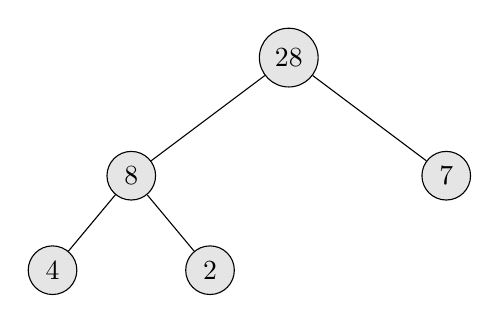
\begin{tikzpicture}[
				level/.style={sibling distance=40mm/#1},
				every node/.style={circle, draw, fill=black!10},
				level 1/.style={level distance=15mm},
				level 2/.style={level distance=12mm},
				level 3/.style={level distance=10mm}
			]
			\node {28}
			child {node {8}
				child {node {4}}
				child {node {2}}
			}
			child {node {7}};
		\end{tikzpicture}
	}
	\newline
	\item{
	      In questo caso il nostro $k = 2$ e di conseguenza, il costo totale dell'albero è 36, che è minimo.
	}
\end{enumerate*}
\end{center}


\[
	\begin{bmatrix}
		[0, 4, -, -]            & [0, 2, -, -]            & [0, 7, -, -] \\
		[8, 4, (1, 1), (1, 2)]  & [7, 14, (1, 2), (1, 3)] & [-, -, -, -] \\
		[36, 7, (2, 1), (1, 3)] & [-, -, -, -]            & [-, -, -, -] \\
	\end{bmatrix}
\]



\subsection{Pseudocodice}